\documentclass[14pt]{beamer}
\title[CP01.13 BC]{COJ :: Getting Started With Java}
\author[TS]{TalentSprint}
\institute[L\&D]{Licensed To Skill}
\date{Version 1.0.4}
\usefonttheme{serif}
\usecolortheme{orchid}
\usepackage{bookman}
\usepackage{hyperref}
\usepackage[T1]{fontenc}
\usepackage{graphicx}
\usepackage{listings}
\lstset{language=Java,numbers=left, numberstyle=\tiny, basicstyle=\footnotesize, numbersep=10pt, showstringspaces=false, breaklines=true,keepspaces=true, columns=flexible}
\beamertemplateballitem
\graphicspath{{../../Images/}}
\usebackgroundtemplate{
\includegraphics[width=\paperwidth]{TS-Logo.jpg}}

\begin{document}
\begin{frame}
  \titlepage
\end{frame}
\begin{frame}{Classes, Objects \& Constructor}
The content in this presentation is aimed at teaching  learners to:
 \begin{itemize}
  \item Define class and object
  \item Differentiate class and object
  \item Create simple java classes, construct and use java objects
  \item Define Constructor
  \item Explain the need for Constructor 
  \item Create Constructors and Parameterized Constructors
  \item Use ``this'' keyword
 \end{itemize}
\end{frame}

\begin{frame}{Classes, Objects \& Constructor}
The Dice Game
\begin{center}
    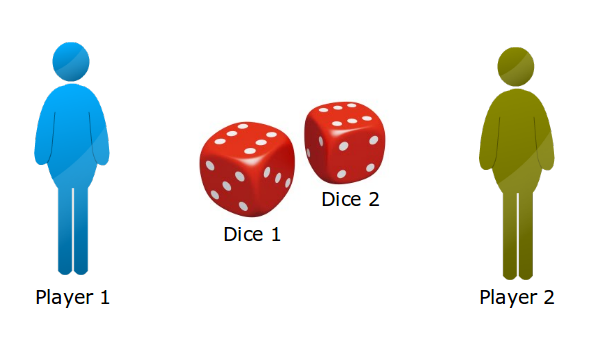
\includegraphics[scale=0.4]{COJ-M01-S03-Image1.png}
  \end{center}
\end{frame}
\begin{frame}{Classes, Objects \& Constructor}
\begin{center}
        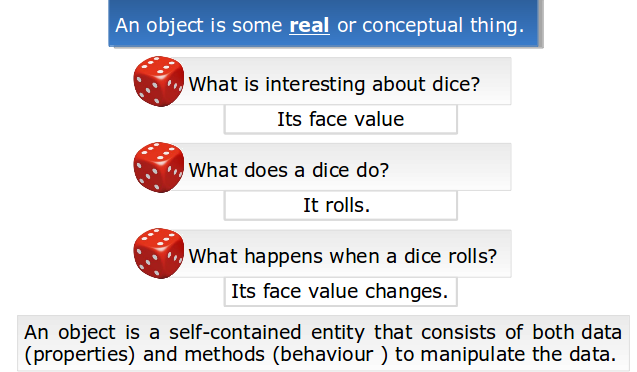
\includegraphics[scale=0.5]{COJ-M01-S03-Image2.png}
          \end{center}
      \end{frame}

      \begin{frame}{Classes, Objects \& Constructor}
      \begin{center}
              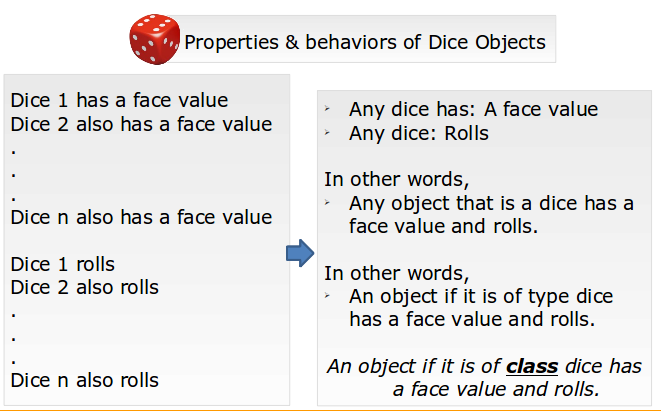
\includegraphics[scale=0.5]{COJ-M01-S03-Image3.png}
                \end{center}
            \end{frame}
            \begin{frame}{Classes, Objects \& Constructor}
            \begin{center}
                    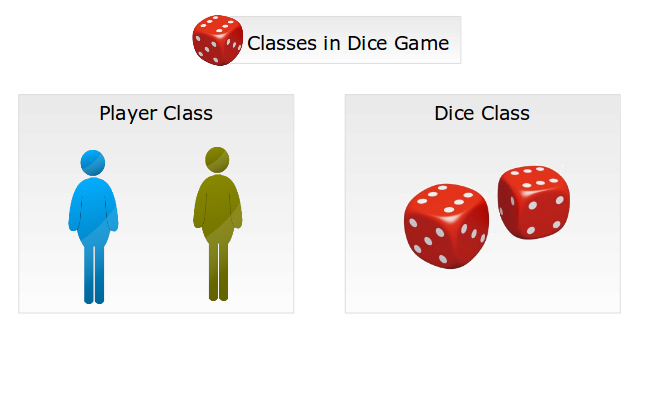
\includegraphics[scale=0.5]{COJ-M01-S03-Image4.png}
                      \end{center}
                  \end{frame}
                  \begin{frame}{Classes, Objects \& Constructor}
                  \begin{tabular}{l l}
                      \begin{minipage}{0.65\textwidth}\end{minipage}
                      &
                      \begin{minipage}{0.25\textwidth}
                          
\includegraphics[scale=.6]{COJ-M01-S03-Image5.png}
                      \end{minipage}
                  \end{tabular}
                  \begin{block}{}
                      A class is a description of a set of objects that share the same attributes and behaviour (operations)
                  \end{block}
              \end{frame}
              \begin{frame}{Classes, Objects \& Constructor}
              Recall the following definitions of abstraction and explain the connect between abstraction and class:
              \begin{tabular}{l l}
                  \begin{minipage}{0.65\textwidth}
                      What is class?
                  \end{minipage}
                  &
                  \begin{minipage}{0.25\textwidth}
                      
\includegraphics[scale=.6]{COJ-M01-S03-Image5.png}
                  \end{minipage}
              \end{tabular}
          \end{frame}
          %\end{document}
          \begin{frame}{Classes, Objects \& Constructor}
          \begin{center}
                  
\includegraphics[scale=0.3]{COJ-M01-S03-Image6.png}
                    \end{center}
                    List out the properties \& behaviors of Player class.

                    Hint : 
                    What is interesting about player?
                    What does a player do?
                \end{frame}
\begin{frame}{Classes, Objects \& Constructor}
\begin{center}
Properties \& Behaviors of Classes in Dice Game
\end{center}
\begin{center}
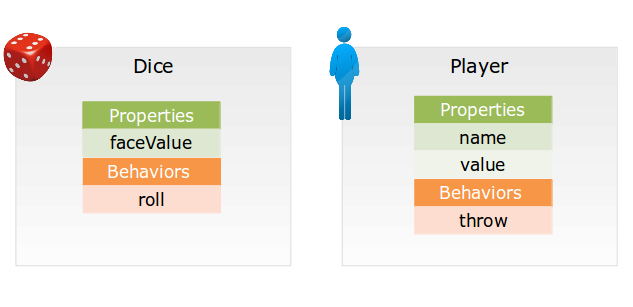
\includegraphics[scale=0.5]{COJ-M01-S03-Image7.png}
\end{center}
\end{frame}


\begin{frame}{Classes, Objects \& Constructor}
\begin{center}
    Properties \& Behaviors of Dice Class
    \end{center}
\begin{center}
    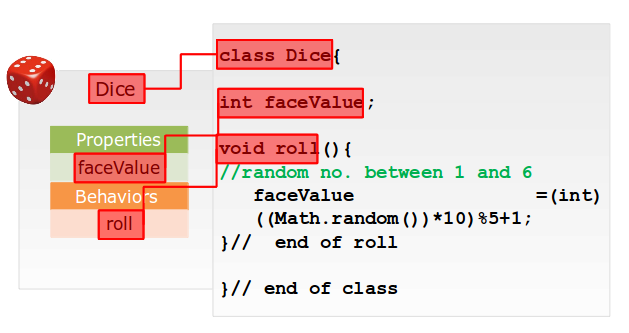
\includegraphics[scale=0.5]{COJ-M01-S03-Image8.png}
\end{center}
\end{frame}
\begin{frame}{Classes, Objects \& Constructor}
\begin{center}
    Properties \& Behaviors of Player Class     
        \end{center}
        \begin{center}
                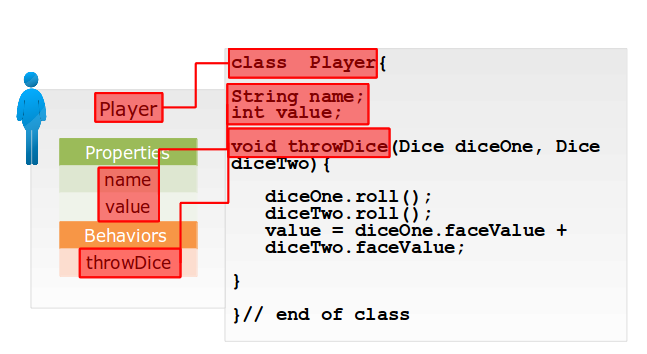
\includegraphics[scale=0.5]{COJ-M01-S03-Image9.png}
            \end{center}
        \end{frame}
      
\begin{frame}{Classes, Objects \& Constructor}
\begin{block}{}
    Programmatic definition of Class
\end{block}
A class is a representation for a set of objects that are data abstractions with an interface of named operations (methods) and hidden local state (attributes).
\end{frame}
\begin{frame}{Classes, Objects \& Constructor}
Behavior in an O-O program
\begin{itemize}
    \item In Object-oriented programming, programs are organized as cooperative collections of objects.
    \item Each object represents an instance of some class.
    \item Objects communicate by passing messages (by calling methods).
        \begin{itemize}
    \item A message is always given to some object. 
    \item The response to a message depends upon the class of the Object.
\end{itemize}
\end{itemize}
\end{frame}
\begin{frame}{Classes, Objects \& Constructor}

\begin{itemize}
\item All messages have three identifiable parts.
    \end{itemize}
    \begin{center}
        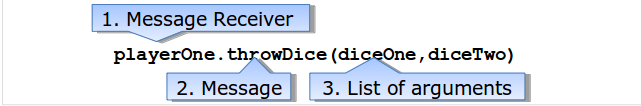
\includegraphics[scale=0.5]{COJ-M01-S03-Image10.png}
                    \end{center}
\end{frame}

\begin{frame}{Classes, Objects \& Constructor}
Making Objects Collaborate

\begin{block}{}
   Steps in making objects collaborate with each other:
\end{block}
\begin{block}{Step 1}
    Define Classes
\end{block}

\begin{block}{Step 2}
     Create Objects
    \end{block}

    \begin{block}{Step 3}
             Pass Messages
                 \end{block}

\end{frame}


\begin{frame}[fragile]{Classes, Objects \& Constructor}
Dice Game Class and main method
\begin{lstlisting}[numbers=none]
class DiceGame {
    public static void main (String args [] ) {
        Dice diceOne;
        diceOne = new Dice();
        // create diceTwo object
        Player playerOne;
        playerOne = new Player();
        playerOne.throwDice(diceOne,diceTwo);
\end{lstlisting}
\end{frame}        
\begin{frame}[fragile]{Classes, Objects \& Constructor}
\begin{lstlisting}[numbers=none]
        // create playerTwo object
        // ask playerTwo to throwDice
        if (playerOne.value > playerTwo.value) {
            System.out.println("Player1 Wins");
        }
        else {
            System.out.println("Player2 Wins");
        }
    }// end of main(
}//end of class DiceGame
\end{lstlisting}
\end{frame}
\begin{frame}{Classes, Objects \& Constructor}
Defining a Class
\begin{center}
            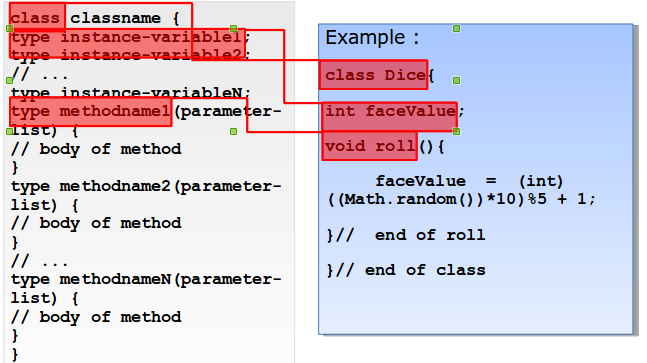
\includegraphics[scale=0.5]{COJ-M01-S03-Image11.png}
                                \end{center}
\end{frame}

\begin{frame}{Classes, Objects \& Constructor}
\begin{block}{}
    <modifier>   <data type>    <name> 
\end{block}

\begin{center}
    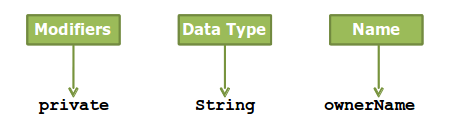
\includegraphics[scale=0.5]{COJ-M01-S03-Image12.png}
    \end{center}
\end{frame}


\begin{frame}{Classes, Objects \& Constructor}
\begin{block}{}
   <modifier>  <return type>  <method name> ( <paramaters> )  \{  
       <statements>
   \} 
\end{block}

\begin{center}
  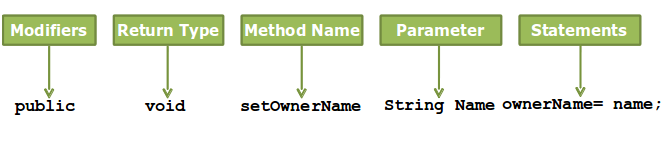
\includegraphics[scale=0.5]{COJ-M01-S03-Image13.png}
\end{center}
\end{frame}
\begin{frame}{Classes, Objects \& Constructor}
Creating Objects
\begin{center}
      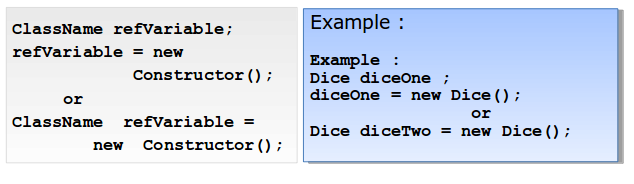
\includegraphics[scale=0.5]{COJ-M01-S03-Image14.png}
  \end{center}
  \end{frame}

  \begin{frame}[fragile]{Classes, Objects \& Constructor}
  Using Objects
  \begin{lstlisting}[numbers=none]
  Dice diceOne = new Dice();
  diceOne.roll();
  int value = diceOne.faceValue();
  \end{lstlisting}
\end{frame}
\begin{frame}[fragile]{Classes, Objects \& Constructor}
  Using Objects
    
  There is one more object in the game. It is the diceGame object itself. Because every object in Java has to belong to some class, let's define the DiceGame class.

  \begin{block}{}
      An object is some real or conceptual thing.
  \end{block}
\end{frame}  
\begin{frame}[fragile]{Classes, Objects \& Constructor}
Properties \& Behaviors of Dice Game Classes
  \begin{center}
  
\includegraphics[scale=0.5]{COJ-M01-S03-Image15.png}
  \end{center}

\begin{lstlisting}[numbers=none]
class DiceGame {
    Player playerOne, playerTwo;
    Dice Diceone, DiceTwo;
    void play() {
        diceOne = new Dice();
        diceTwo = new Dice();
\end{lstlisting}
\end{frame}
\begin{frame}[fragile]{Classes, Objects \& Constructor}
\begin{lstlisting}[numbers=none]
        playerOne = new Player();
        playerTwo = new Player();
        playerOne.throwDice(diceOne,diceTwo);
        playerTwo.throwDice(diceOne,diceTwo);
        if (playerOne.value > playerTwo.value) {
            System.out.println("Player  One Wins");
        }
        else {
            System.out.println("Player  Two Wins");
        }   
    }// end of play()
                                                                            
}//end of class
\end{lstlisting}
\end{frame}
\begin{frame}[fragile]{Classes, Objects \& Constructor}
Create the main method for the DiceGame class and complete the game.
\end{frame}
\begin{frame}[fragile]{Classes, Objects \& Constructor}
Using Objects

\begin{center}
      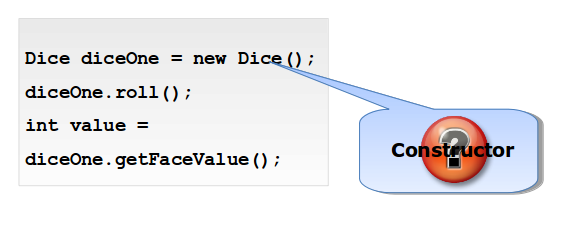
\includegraphics[scale=0.5]{COJ-M01-S03-Image16.png}
\end{center}
\end{frame}

 \begin{frame}[fragile]{Classes, Objects \& Constructor}
    \begin{block}{}
        Constructor
    \end{block}
    \begin{itemize}
        \item Is a function that is implicitly invoked when a new object is created.
        \item Performs the necessary actions in order to initialize the object.
        \item Is a special function with the same name as the class.
    \end{itemize}
    Example:
    Using Objects

    \begin{lstlisting}[numbers=none]
class  Car {
    public Car(){ // this is constructor
    . . . 
    }
}
\end{lstlisting}
\end{frame}

\begin{frame}[fragile]{Classes, Objects \& Constructor}


\begin{center}
          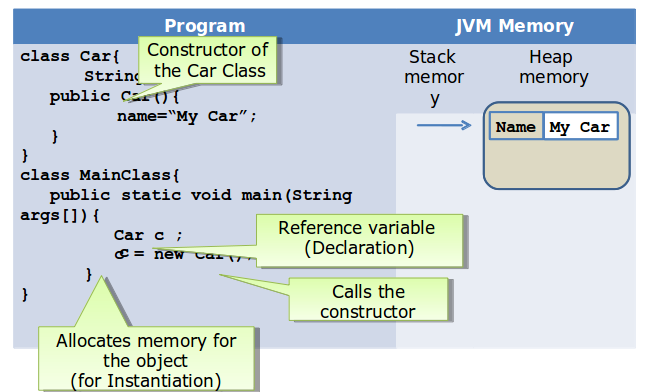
\includegraphics[scale=0.5]{COJ-M01-S03-Image17.png}
                  \end{center}
\end{frame}


\begin{frame}{Classes, Objects \& Constructor}

\begin{block}{}
    Constructor
\end{block}
\begin{center}
              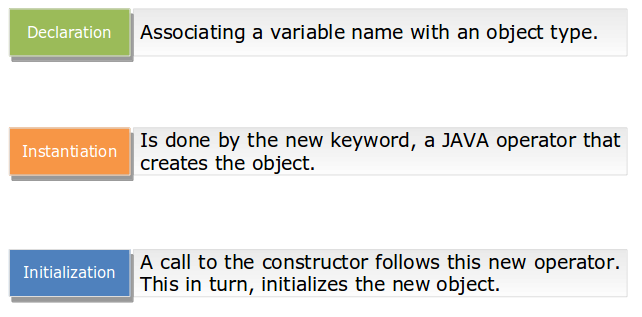
\includegraphics[scale=0.5]{COJ-M01-S03-Image18.png}
                                \end{center}
\end{frame}
                                                  

\begin{frame}[fragile]{Classes, Objects \& Constructor}


\begin{center}
              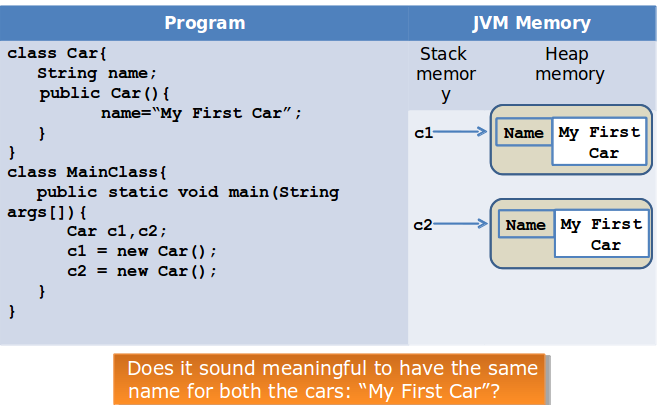
\includegraphics[scale=0.5]{COJ-M01-S03-Image19.png}
                                \end{center}
\end{frame}

\begin{frame}[fragile]{Classes, Objects \& Constructor}
\begin{center}
  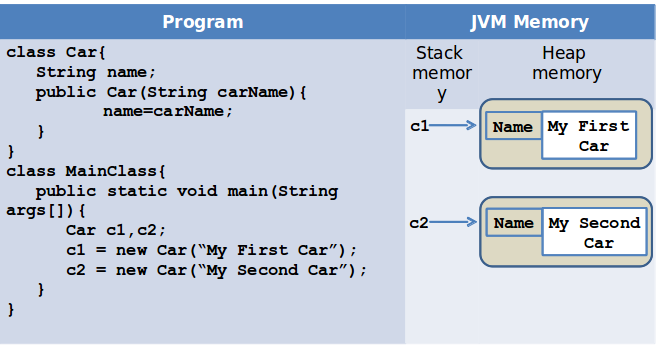
\includegraphics[scale=0.5]{COJ-M01-S03-Image20.png}
\end{center}
\end{frame}
\begin{frame}{Classes, Objects \& Constructor}
\begin{center}
  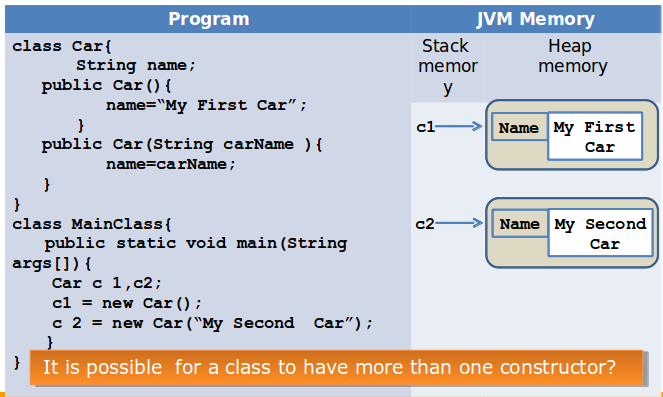
\includegraphics[scale=0.5]{COJ-M01-S03-Image21.png}
  \end{center}
  \end{frame}
\begin{frame}{Classes, Objects \& Constructor}

\begin{center}
            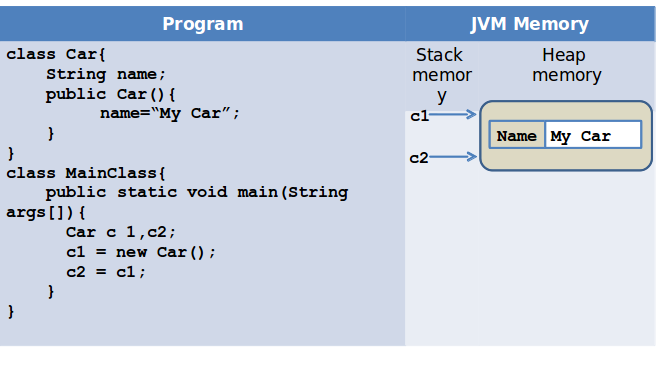
\includegraphics[scale=0.5]{COJ-M01-S03-Image22.png}
              \end{center}
                \end{frame}
\begin{frame}{Classes, Objects \& Constructor}
\begin{center}
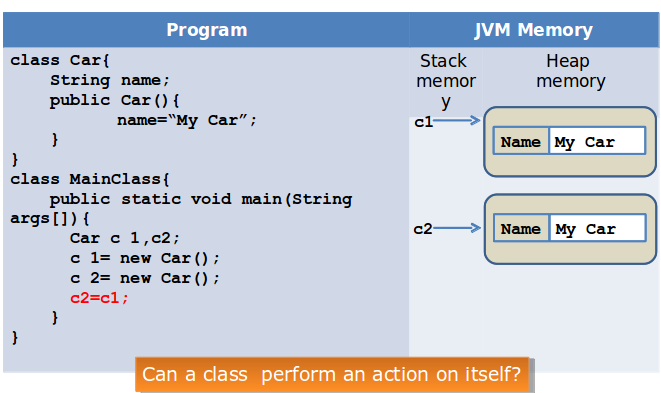
\includegraphics[scale=0.5]{COJ-M01-S03-Image23.png}
\end{center}
\end{frame}

\begin{frame}{Classes, Objects \& Constructor}
\begin{center}
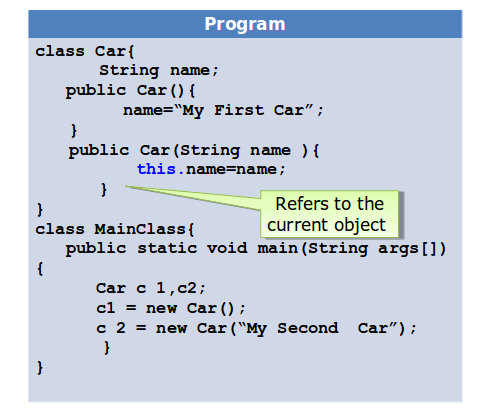
\includegraphics[scale=0.5]{COJ-M01-S03-Image24.png}
\end{center}
\end{frame}
\begin{frame}{Classes, Objects \& Constructor}
\begin{center}
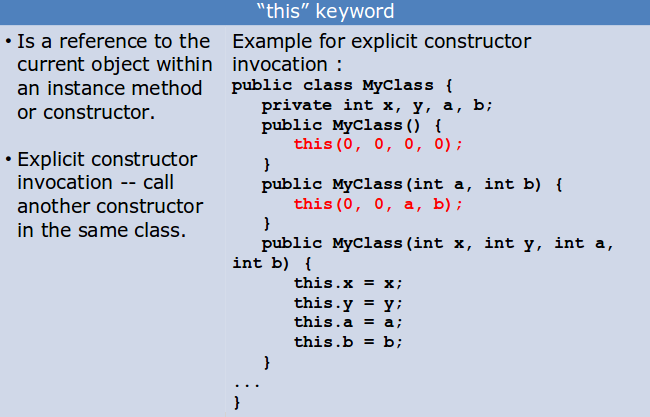
\includegraphics[scale=0.5]{COJ-M01-S03-Image25.png}
\end{center}
\end{frame}
\begin{frame}[fragile]{Classes, Objects \& Constructor}
\begin{block}{}
Will this work?
\end{block}
\begin{lstlisting}[numbers=none]
Class Test{
   // no constructor
   int value=10;
   void display(){
      System.out.println(“Value is : ”+value);
   }
}
class MainClass{
   public static void main(String args[]){
      Test test = new Test(); //  creating  object with constructor Test()
      test.display();
   }
}
\end{lstlisting}
\end{frame}
\begin{frame}[fragile]{Classes, Objects \& Constructor}
\begin{block}{}
What if no constructor is defined  in a class ?
\end{block}
\begin{itemize}
\item  At the time of compilation the Java Compiler will insert an empty Definition Of Default Constructor to the java class and then it will compile the program.
\item The empty Definition Of Default Constructor of any class will be as follows:
\end{itemize}
\begin{lstlisting}[numbers=none]
public class-name(){} 
\end{lstlisting}
\end{frame}
\begin{frame}{Classes, Objects \& Constructor}
\begin{center}
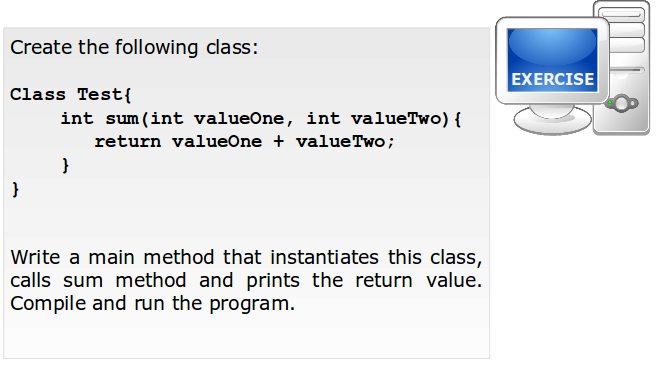
\includegraphics[scale=0.5]{COJ-M01-S03-Image26.png}
\end{center}
\end{frame}
\begin{frame}{Classes, Objects \& Constructor}
\begin{center}

\includegraphics[scale=0.5]{COJ-M01-S03-Image27.png}
\end{center}
\end{frame}
\end{document}

